\chapter{Desenvolvimento} \label{cap:desenvolvimento}

\section{Hardware}

    Para a impressão dos blocos foi utilizado a impressora 3D SnapMaker com o filamento branco no material PETG. Foi impresso uma peça nas medidas definidas no capitulo 3 para testes de material e tamanho conforme apresentado na Figura \ref{figura:teste_bloco}.
    
    \begin{figure}[H]
        \caption{Teste de tamanho e material do bloco físico}
        \centering
        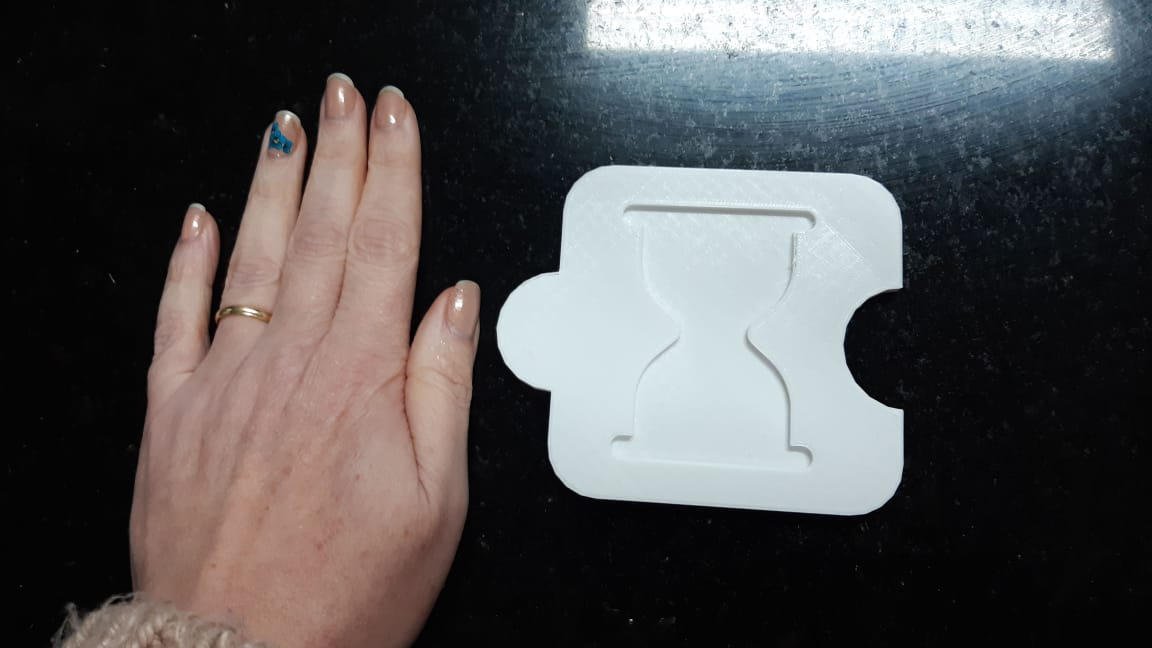
\includegraphics[width=\linewidth]{Imagens/Cap4/teste_bloco.jpeg}
        \legend{\small{Fonte: o autor (2020)}}
        \label{figura:teste_bloco}
    \end{figure}
    
    Nos testes, verificamos que o material escolhido estava dentro dos padrões aceitáveis, mantendo a peça conforme o planejado. Analisamos o tamanho da peça impressa e identificamos que estava muito grande, podendo dificultar a captura da solução pela criança. O tamanho do bloco foi reduzido para 7cm x 7cm x 5mm e um novo teste foi realizado, obtendo sucesso.
    
    Para facilitar a identificação dos blocos numéricos, alteramos o encaixe  do bloco de loop para que o bloco numérico possa encaixar lateralmente, deixando todos os blocos com encaixes laterais conforme apresentado na Figura \ref{figura:alteracao_bloco_numerico}.
    
    \begin{figure}[H]
        \caption{Alteração do bloco numérico}
        \centering
        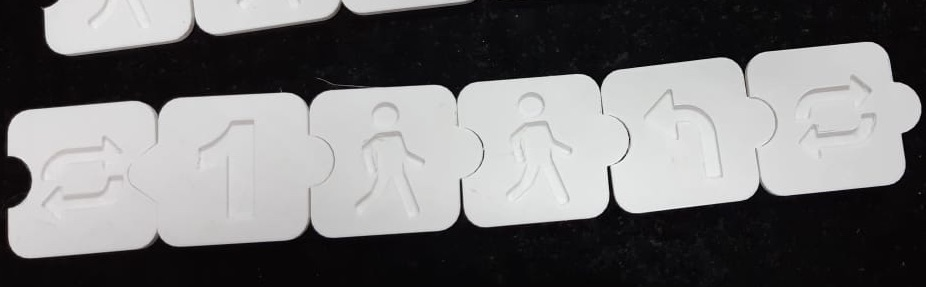
\includegraphics[width=\linewidth]{Imagens/Cap4/alteracao_bloco_numerico.jpg}
        \legend{\small{Fonte: o autor (2020)}}
        \label{figura:alteracao_bloco_numerico}
    \end{figure}
    
    As peças, impressas na cor branca, foram coloridas utilizando tinta de tecido nas cores verde, amarelo, laranja e roxo conforme apresentado na Figura \ref{figura:blocos_pintados}
    
    \begin{figure}[H]
        \caption{Alteração do bloco numérico}
        \centering
        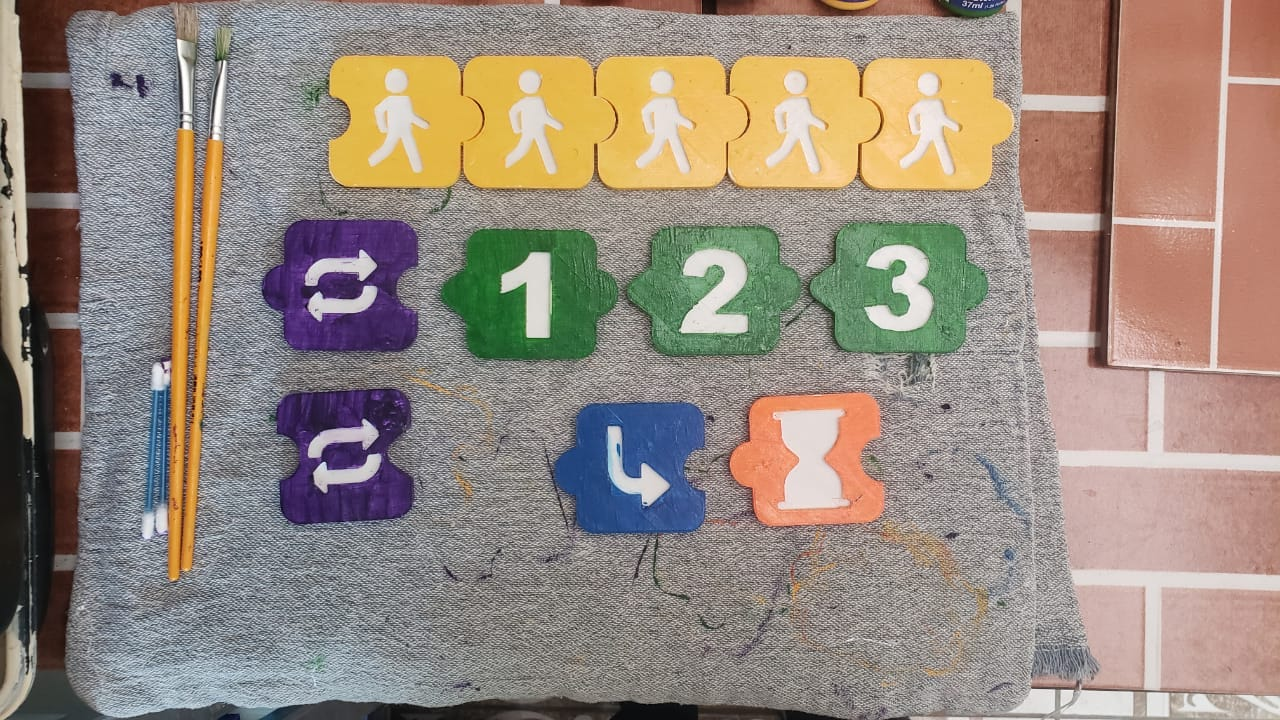
\includegraphics[width=\linewidth]{Imagens/Cap4/blocos_pintados.jpeg}
        \legend{\small{Fonte: o autor (2020)}}
        \label{figura:blocos_pintados}
    \end{figure}

\section{Software}

Para apresentar todos os softwares que compõem o aplicativo, esta seção é dividida em três subseções: jogo, software de reconhecimento dos blocos e por fim integração dos softwares.

    \subsection{Jogo}
    
    Para o desenvolvimento do jogo foi utilizado a engine Unity 3D, assets gratuitos obtidos no site Flaticon e o editor de código Visual Studio Code, a linguagem de programação utilizada foi C\# (CSharp), o jogo foi desenvolvido para smartphones com a plataforma Android 5.0 ou superior, sendo necessário acesso a internet para que o mesmo funcione.
    
    Ao iniciar o aplicativo, é apresentado para a criança a tela inicial. O fluxograma apresentado na Figura \ref{figura:fluxo_telas} mostra o fluxo de telas do menu apresentado.
    
    \begin{figure}[H]
        \caption{Fluxo de Telas do menu}
        \centering
        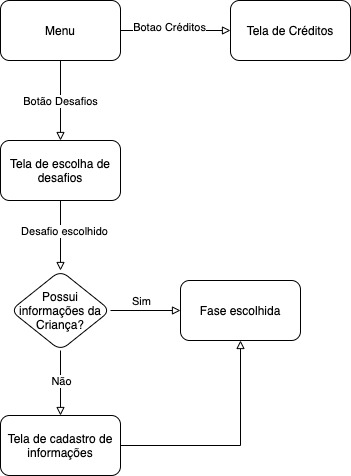
\includegraphics[width=10cm]{Imagens/Cap4/fluxo_menu.jpg}
        \legend{\small{Fonte: o autor (2020)}}
        \label{figura:fluxo_telas}
    \end{figure}
    
    Na tela inicial, apresentada na Figura \ref{figura:menu_final}, a criança pode ser direcionada para a tela de créditos e desafios, resolvidos e disponíveis. 
    
    \begin{figure}[H]
        \caption{Menu do Jogo}
        \centering
        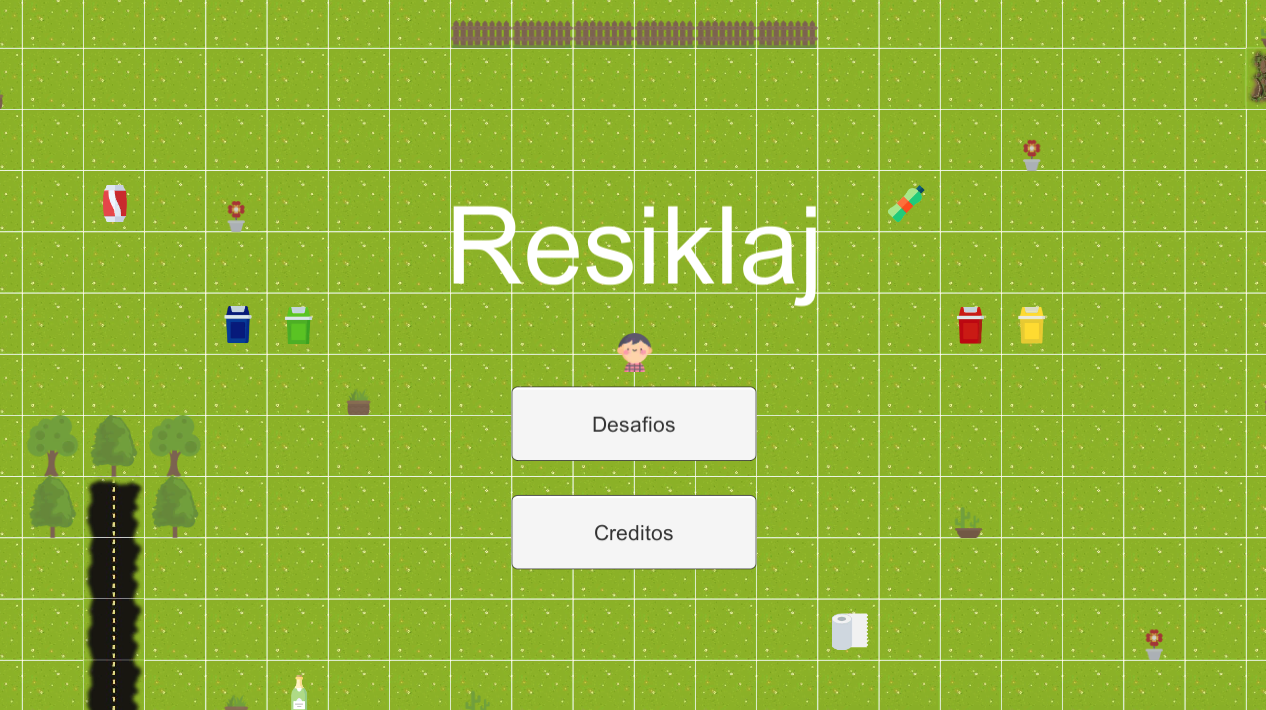
\includegraphics[width=14cm]{Imagens/Cap4/menu_final.png}
        \legend{\small{Fonte: o autor (2020)}}
        \label{figura:menu_final}
    \end{figure}
    
    Ao jogar pela primeira vez é solicitado duas informações, nome e idade, para identificar a criança, conforme apresentado na Figura \ref{figura:tela_final_cadastro}. Essas informações são salvas localmente no smartphone e serão enviadas para o servidor junto com o envio de cada solução dos desafios, todas as soluções, corretas ou não, serão salvas no banco de dados para análise estatística e desempenho de cada criança.
    
    \begin{figure}[H]
        \caption{Tela de Cadastro}
        \centering
        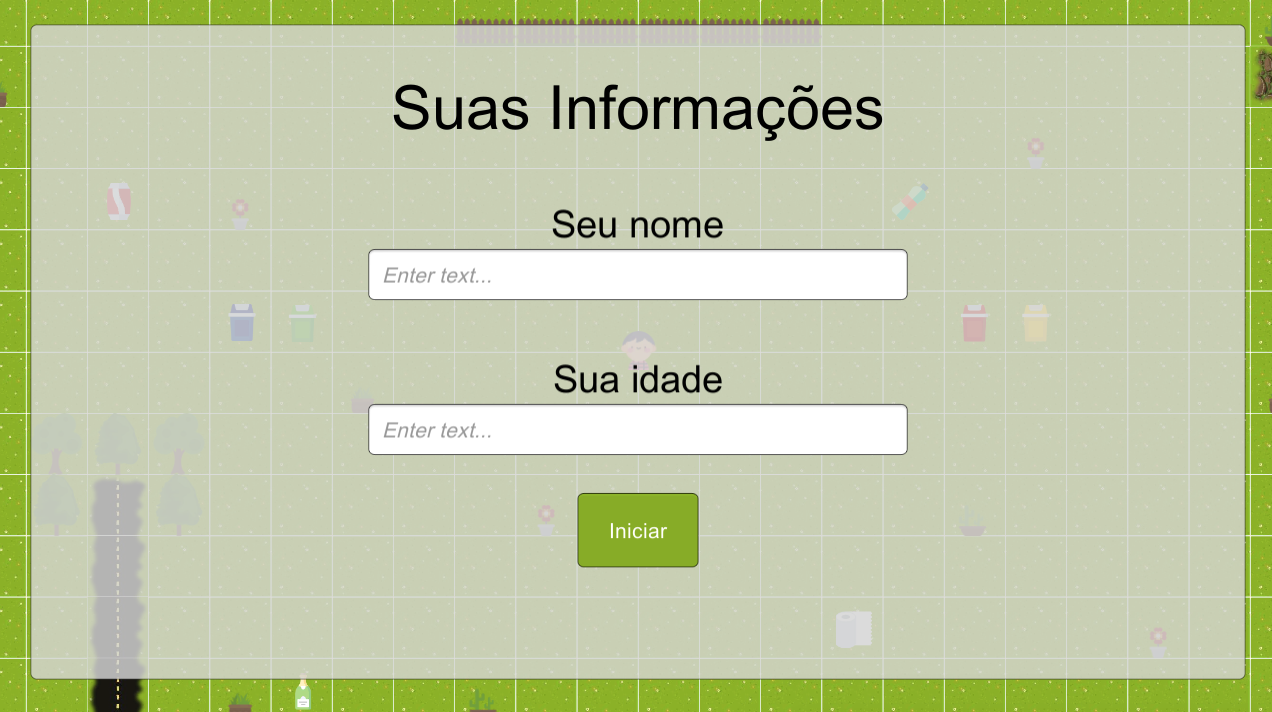
\includegraphics[width=14cm]{Imagens/Cap4/tela_final_cadastro.png}
        \legend{\small{Fonte: o autor (2020)}}
        \label{figura:tela_final_cadastro}
    \end{figure}
    
    O jogo possui 4 fases, cada uma delas apresenta um novo bloco lógico juntamente com o descarte correto de um tipo de lixo. Para a estruturação delas foi utilizado o componente Grid da Unity. Todas as fases possuem dois grids, um para o chão e outro para a decoração e cada um possui seu próprio \textit{titlemap}. Os objetos das fases como lixos, lixeiras e personagem são tratados individualmente.
    
    \subsubsection{Objetos e Controladores}
    
    O jogo possui dois objetos bases, o lixo e a lixeira. O lixo possui 4 parâmetros apresentados na Figura \ref{figura:parametros_lixo}. O parâmetro \textit{Trash Type} representa o tipo do Lixo (Papel, Plástico, Metal e Vidro), o parâmetro \textit{Collected} representa se o lixo foi coletado no cenário, o \textit{Discarted} representa se o lixo foi descartado e o \textit{Discarted Correctly} representa se o lixo foi descartado na lixeira correta. 
    
    \begin{figure}[H]
        \caption{Parâmetros do Objeto Lixo Papel}
        \centering
        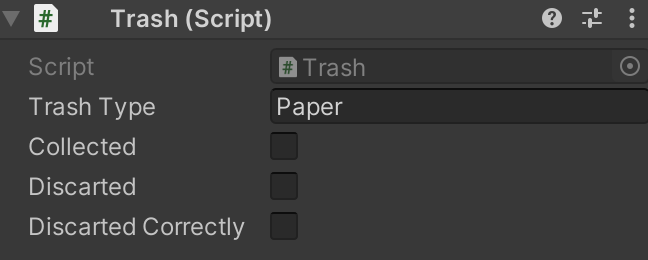
\includegraphics[width=10cm]{Imagens/Cap4/parametros_lixo.png}
        \legend{\small{Fonte: o autor (2020)}}
        \label{figura:parametros_lixo}
    \end{figure}
    
    A lixeira possui apenas um parâmetro conforme apresentado na Figura \ref{figura:parametro_lixeira}, o \textit{Trash Type Accepted} que representa qual tipo de lixo aquela lixeira aceita.
    
    \begin{figure}[H]
        \caption{Parâmetros do Objeto Lixeira Metal}
        \centering
        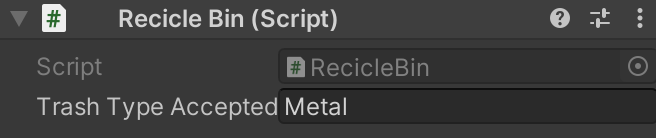
\includegraphics[width=10cm]{Imagens/Cap4/parametro_lixeira.png}
        \legend{\small{Fonte: o autor (2020)}}
        \label{figura:parametro_lixeira}
    \end{figure}
    
    O gerenciamento da câmera do dispositivo é feita através de um controlador, ele é responsável por controlar as funções básicas da câmera (abrir, fechar e tirar foto) e inciar o processo de envio da imagem para que ela possa ser interpretada pelo software de reconhecimento.
    
    Cada fase do jogo, possui uma quantidade especifica de objetos (Lixo e lixeiras), de acordo com seu nível de dificuldade, e um controlador, apresentado na Figura \ref{figura:controlador_fases}, responsável por gerenciar o envio, compilação e execução da solução, além de identificar quando o a solução proposta está correta ou não. 
    
    \begin{figure}[H]
        \caption{Controlador das Fases}
        \centering
        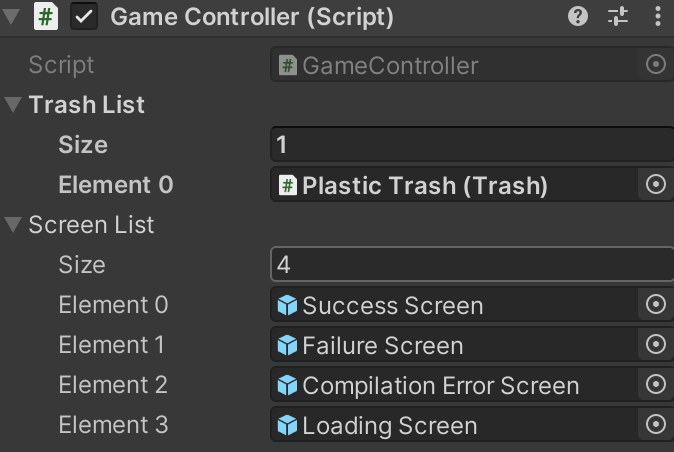
\includegraphics[width=10cm]{Imagens/Cap4/controlador_fases.png}
        \legend{\small{Fonte: o autor (2020)}}
        \label{figura:controlador_fases}
    \end{figure}
    
    Após receber o retorno do software de reconhecimento, a lista com os blocos passa por um compilador que verifica se a solução enviada foi estruturada corretamente, esse processo inclui a verificação da quantidade de loops e blocos numéricos presentes na solução. Após a conclusão, bem sucedida, do processo de compilação, é iniciado o processo de execução e logo em seguida a identificação se a solução enviada atingiu os objetivos da fase. Para que a identificação seja possível, o controlador possui uma lista dos lixos dispostos no cenário e valida se todos os lixos foram coletados e descartados corretamente.
    
    
    \subsection{Software de reconhecimento dos blocos}
    
    O software de reconhecimento dos blocos é uma API, isto é, uma interface de programação de aplicações,  desenvolvida em Python. Os principais módulos utilizados no desenvolvimento deste software são OpenCV, numpy, pytesseract e flask.

    Com base no referencial teórico deste trabalho sobre visão computacional, foi desenvolvida uma API capaz de receber uma imagem dos blocos, reconhecê-los com base nas classes de blocos propostos e por fim retornar os blocos contidos na imagem submetida no formato JSON. O software de reconhecimento é limitado às seguintes restrições:
    
        \begin{itemize}
        \item Os blocos a serem reconhecidos devem exclusivamente ser desenvolvidos pelos pesquisadores e desenvolvedores deste trabalho, qualquer cópia poderá não funcionar como proposto;
        \item A imagem deve estar iluminada adequadamente (sem sombras);
        \item As cores do plano no qual os blocos estiverem dispostos devem ser diferentes das cores de qualquer um dos blocos (preferencialmente branco);
        \item A imagem deve ser capturada de forma perpendicular à superfície na qual os blocos estejam dispostos;
       \item Os blocos a serem reconhecidos devem estar centralizados na imagem e não podem estar cortados;
      \item Os blocos a serem reconhecidos não podem estar sobrepostos.
    \end{itemize}

    As etapas do desenvolvimento do algoritmo de reconhecimento dos blocos estão ilustradas no fluxograma na Figura \ref{figura:fluxo}. 
    Nas subseções subsequentes está descrito, com exemplos, o funcionamento de cada etapa do software de reconhecimento dos blocos.
    
    \begin{figure}[H]
        \caption{Fluxograma de Reconhecimento dos Blocos}
        \centering
        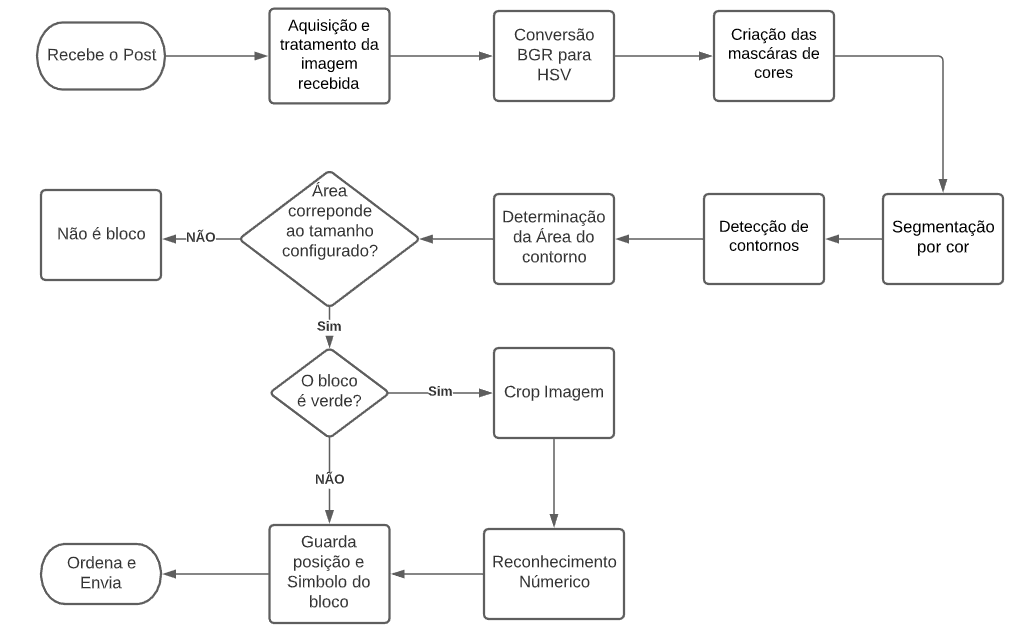
\includegraphics[width=\linewidth]{Imagens/Cap4/fluxo.PNG}
        \legend{\small{Fonte: o autor (2020)}}
        \label{figura:fluxo}
    \end{figure}


    \subsubsection{Aquisição}
    
    Após o recebimento da imagem através do protocolo http POST, é necessário converter a imagem de bytes para um vetor numpy através do comando \textit{fromstring} do módulo numpy, pois é neste formato que o módulo OpenCV é capaz de ler as imagens. 
    
    Uma etapa comum em visão computacional é o redimensionamento  das imagens, porém neste caso não se fez necessário o redimensionamento pois as imagens já são enviadas em um tamanho pré definido pelo aplicativo jogo.

    \subsubsection{Conversão de BGR para HSV}
    O padrão HSV consiste em cor, retratado como \textit{Hue}; a saturação da cor por \textit{Saturation} e por fim o brilho, chamado de \textit{value}, por conta disso possui o nome HSV.
    
    A etapa de conversão de BGR (\textit{blue}, \textit{green} e \textit{red}) para HSV é fundamental, pois é por meio deste padrão que as máscaras, utilizadas para isolar cada cor da imagem é criada. Portanto é por conta desta etapa que a segmentação por cores se torna possível.

    
    \subsubsection{Segmentação Por Cor}
    Nesta etapa a imagem inicial se desfaz em N imagens, onde N  é o número de blocos distintos na imagem submetida para reconhecimento dos blocos.
    
    Nesta etapa o algoritmo compara a imagem submetida para o reconhecimento com uma máscara e realiza uma filtragem de cores. Estas máscaras são criadas a partir de 3 parâmetros, o máximo de valores BGR para uma determinada cor, o mínimo valores BGR para a mesma cor, e por fim com os valores da imagem gerada através da conversão BGR para HSV da etapa anterior. 
    
    No momento em que a imagem passa por este filtro de segmentação de cor, as componentes de cor que não fazem parte do espectro definido como máximo e mínimo são zeradas, resultando em uma imagem com apenas a cor que faz parte do espectro especificado, como ilustrado nas Figuras \ref{figura:ex1_original} e \ref{figura:ex1_tratado}, nas quais, pode-se ver o antes e depois da segmantação da cor laranja de uma imagem com diversos blocos de cores distintas.
    
    \begin{figure}[H]
        \caption{Exemplo de segmentação por cor - original}
        \centering
        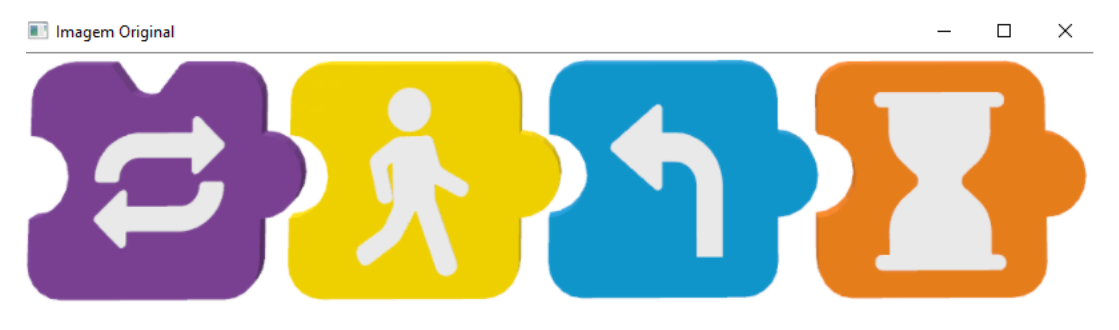
\includegraphics[width=\linewidth]{Imagens/Cap4/ex1_original.PNG}
        \legend{\small{Fonte: o autor (2020)}}
        \label{figura:ex1_original}
    \end{figure}
    
    
    \begin{figure}[H]
        \caption{Exemplo de segmentação por cor - após tratamento}
        \centering
        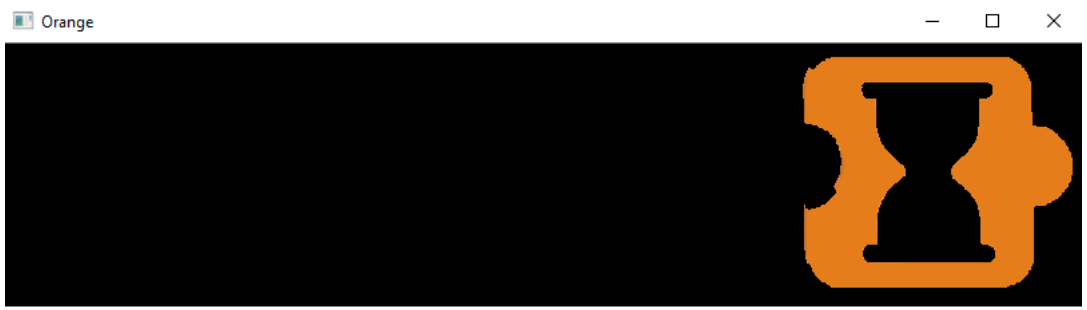
\includegraphics[width=\linewidth]{Imagens/Cap4/ex1_tratado.PNG}
        \legend{\small{Fonte: o autor (2020)}}
        \label{figura:ex1_tratado}
    \end{figure}
    
    \subsubsection{Detecção de Contorno}
    Nesta etapa, espera-se que as imagens estejam com as cores isoladas para que passem pelo processo de detecção de contorno da melhor maneira possível. Esta etapa consiste basicamente na detecção de bordas das imagens provenientes da etapa anterior.

    Através das máscaras HSV geradas, é realizada uma busca por contornos das cores que fazem parte do espectro determinado para cada cor.
    
    Depois que os contornos são encontrados, verifica-se se algum contorno possui área maior que um valor X, o qual varia dependendo do bloco, como ilustrado na Tabela \ref{table:area_values}. Se a área do contorno for maior que o valor pré determinado, o algoritmo assume, considerando a limpeza de ruídos feita na etapa de segmentação de cores e o tamanho da área encontrado nesta etapa, que aquela seção da imagem corresponde a um bloco da cor da máscara testada. Portanto por meio desta etapa, já é possível reconhecer os blocos que possuem somente uma cor para um símbolo, isto é, laranja - esperar, amarelo - caminhar, azul - virar e roxo - repetir.
    
    \begin{table}[H]
        \centering
        \caption{Tabela de valor mínimo de área}
        \label{table:area_values}
        \begin{tabular}{ |c|c| } 
         \hline
        Cor     & Mínimo valor de área \\
         \hline
        Azul    & 10000                \\
         \hline
        Amarelo & 7500                 \\
         \hline
        Laranja & 10000                \\
         \hline
        Roxo    & 12500                \\
         \hline
        Verde   & 10000                \\    [0.5ex]    
         \hline
        
        \end{tabular}
        \legend{\small{Fonte: o autor (2020)}}
        
    \end{table}
    
        
    \subsubsection{Reconhecimento Numérico}
    Por fim, para o reconhecimento dos blocos numéricos se faz necessário uma etapa de OCR, ou seja, reconhecimento ótico de caracteres, pois não são possíveis descrevê-los totalmente pelas etapas anteriores, pois além da cor verde, também é preciso determinar seu símbolo.
    
    Antes da etapa de OCR, a imagem passa por uma função de corte, na qual a região do símbolo a ser reconhecido é isolado com objetivo de diminuir possíveis erros da etapa de OCR. Portanto, se um bloco foi identificado como verde, obtém-se, por meio da função de achar contornos,  as coordenadas da região a ser reconhecida pela etapa de OCR e, por meio de suas coordenadas, essa região é cortada da imagem original como ilustrado nas Figuras \ref{figura:ex2_original} e \ref{figura:ex2_tratado}.
    
    \begin{figure}[H]
        \caption{Exemplo Tratamento para OCR - original}
        \centering
        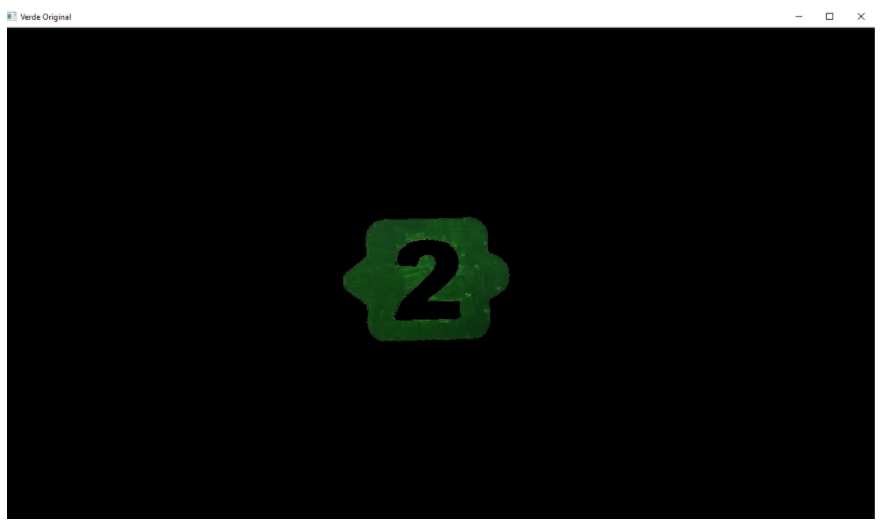
\includegraphics[width=14cm]{Imagens/Cap4/ex2_original.PNG}
        \legend{\small{Fonte: o autor (2020)}}
        \label{figura:ex2_original}
    \end{figure}
    
    
    \begin{figure}[H]
        \caption{Exemplo Tratamento para OCR - após tratamento}
        \centering
        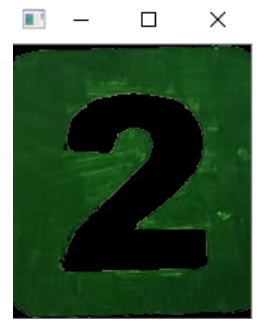
\includegraphics[width=7cm]{Imagens/Cap4/ex2_tratado.PNG}
        \legend{\small{Fonte: o autor (2020)}}
        \label{figura:ex2_tratado}
    \end{figure}
    
    Na etapa do OCR, a imagem cortada é confrontada com uma lista de 10 possíveis valores, números entre 0 e 9, e por meio do módulo de Python \textit{pytesseract} e do software \textit{Tesseract}, o símbolos numéricos dos blocos verdes são reconhecidos.


    \subsubsection{Envio das Informações}
    Durante as etapas anteriores, na medida em que os blocos são reconhecidos, os seus significados e, por meio da função achar contornos, suas coordenadas são armazenadas em uma estrutura de dados Python conhecida com tupla.
    
    Por fim, esta estrutura que contém os blocos e suas respectivas posições na imagem é ordenada baseada nas coordenadas do menor valor de X para o maior valor de X, em outras palavras, da esquerda para a direita da imagem. Esses valores então são  encapsulados em uma estrutura JSON e são enviados como retorno da API para o aplicativo jogo.

    \subsubsection{Testes}
    
    Os primeiros testes foram realizados no decorrer do desenvolvimento do software com uma imagem genérica de um círculo cromático. Esses primeiros testes tinham o objetivo de ver os efeitos das funções do OpenCV em uma imagem com diversas cores.
    
    Após o desenvolvimento do software, foram realizados teste com imagens dos blocos com o objetivo de ajustar os parâmetros das máscaras de segmentação por cor e os tamanhos das áreas mínimas dos contornos para se considerar um bloco. Primeiramente foram realizados testes unitários com as imagens dos protótipos dos blocos reais, cada imagem com apenas um bloco em um fundo branco como ilustrado na Figura \ref{figura:ex_teste}. Nos próximos testes foi utilizado imagens no mesmo padrão de qualidade, porém com sequências de blocos.
       
    \begin{figure}[H]
        \caption{Exemplo de imagem de teste}
        \centering
        
\includegraphics[width=8cm]{Imagens/Cap3/Blocos/Virar.png}
        \legend{\small{Fonte: o autor (2020)}}
        \label{figura:ex_teste}
    \end{figure}
    
    Após o sucessos na primeira bateria de testes, foram realizados testes com imagens mais próximas da realidade, isto é, dos blocos reais em diferentes iluminações e em diferentes superfícies. Os padrões de teste foi o mesmo utilizado na primeira etapa, ou seja, em um primeiro momento os testes foram realizados com imagens com apenas um bloco para somente então imagens com sequências de blocos.
    
    Durante a etapa de testes o algoritmo foi ajustado para reduzir ao máximo erros provocados por fenômenos como sombras, iluminação, cores de superfícies e distâncias dos blocos, porém o software ainda está sujeito a erros se não utilizado com imagens em qualidade adequada, como descrito no início desta seção.    

    \subsection {Integração dos Softwares}
    
    Para a integração dos softwares (jogo e reconhecimento dos blocos), foi utilizado a linguagem Python junto como framework Flask, transformando o software de reconhecimento em uma API com arquitetura REST, o diagrama da Figura \ref{figura:diagrama_acesso_integracao} representa o acesso ao serviço de reconhecimento.
    
    \begin{figure}[H]
        \caption{Diagrama de acesso ao serviço de reconhecimento}
        \centering
        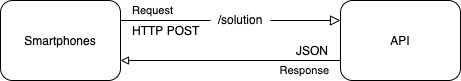
\includegraphics[width=15cm]{Imagens/Cap4/diagrama_acesso_integracao.jpg}
        \legend{\small{Fonte: o autor (2020)}}
        \label{figura:diagrama_acesso_integracao}
    \end{figure}
    
    O Serviço possui 3 rotas, sendo que, somente uma delas possui retorno gráfico ao acessar via navegador. A tabela \ref{tab:rotas} apresenta as rotas do serviço.
    
    \begin{table}[H]
        \centering
        \caption{Tabela de rotas do serviço}
        \label{tab:rotas}
        \begin{tabular}{|c|c|c|}
            \hline
            {Rota} & {Metodos} & {Parâmetros}  \\ \hline
            /solution & POST, PATCH & image, child, rightSolution \\ \hline
            /dashboard & GET & childID \\ \hline
        \end{tabular}
        \legend{\small{Fonte: o autor (2020)}}
    \end{table}
    
    A rota \textit{/solution} é responsável por gerenciar as soluções propostas. O método POST recebe a imagem da solução, através do parâmetro \textit{image}, executa as ações de reconhecimento apresentadas na seção anterior e após isso, salva no banco de dados a solução e as informações da criança, recebidas pelo parâmetro \textit{child}. O método PATCH atualiza se a solução foi ou não correta, usando o parâmetro \textit{rightSolution} em combinação com o parâmetro \textit{child}.
    
    A rota \textit{/dashboard} é responsável por apresentar o relatório para os professores/tutores. O parâmetro \textit{childID} é a identificação da criança a ser visualizada, caso esse parâmetro não seja passado, é apresentado o relatório com todas as crianças.
    
    Na arquitetura criada, a comunicação é sempre iniciada pelo smartphone com o jogo. Como o serviço é segregado do jogo, ele consegue trabalhar de forma independente, podendo se conectar a outros jogos e aplicativos, desde que, o padrão estabelecido para a comunicação seja respeitado. No jogo, não existe possibilidade de trabalhar independente, pois ele necessita do serviço para reconhecer os blocos na solução enviada, tornando obrigatório o acesso a Internet.
    
    \subsubsection{Padrão de comunicação}
    
    Para possibilitar a integração entre o jogo e o software de reconhecimento, foi definido um padrao de resposta da API. A resposta da rota \textit{/solution} para quando é submetido uma solução através do método POST contém um encapsulador, representado pela propriedade \textit{blocks}. Esse encapsulamento da resposta, possibilita a interpretação do JSON recebido na Unity 3D, visto que, para que consiga ser interpretado, todas as propriedades do JSON devem ser traduzidas para classes dentro do jogo, O conteúdo retornado nessa propriedade é uma lista com os objetos que representam os blocos, conforme apresentado na Figura \ref{figura:json_retorno}.
    
    \begin{figure}[H]
        \caption{JSON de retorno}
        \centering
        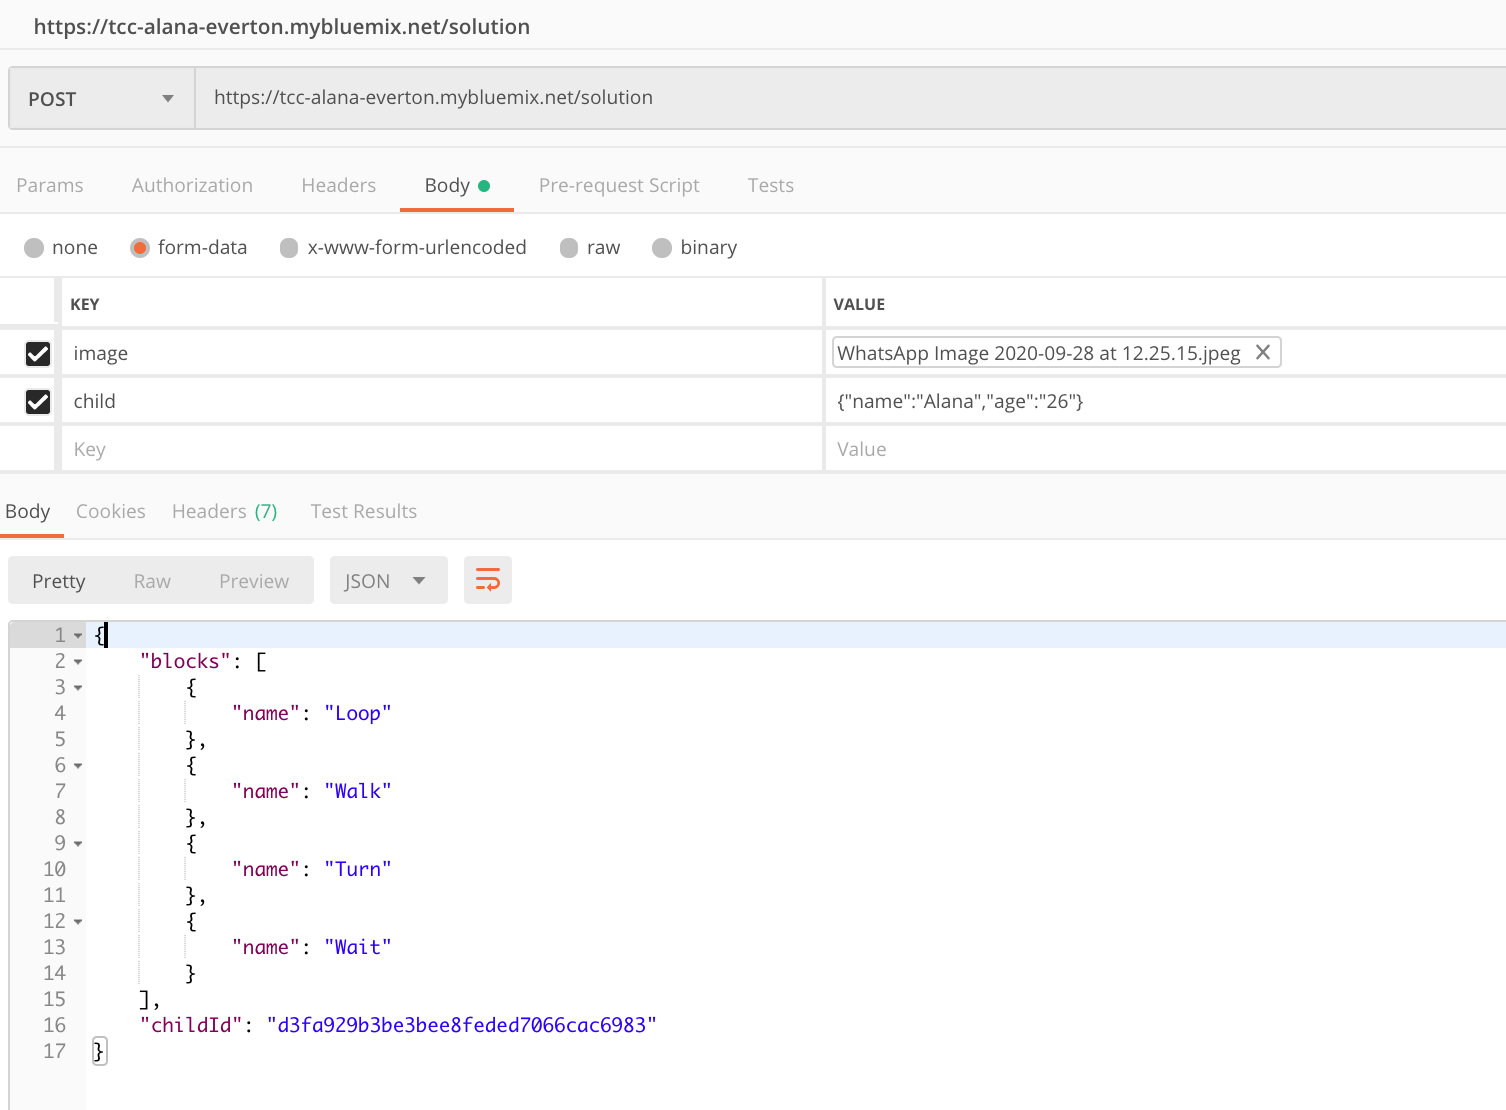
\includegraphics[width=\linewidth]{Imagens/Cap4/json_retorno.png}
        \legend{\small{Fonte: o autor (2020)}}
        \label{figura:json_retorno}
    \end{figure}
    
    O objeto que representa o bloco possui uma propriedade, \textit{name}, que contém o nome do bloco. Caso o bloco identificado seja o bloco numérico, o mesmo retorna o seu respectivo numero precedido da palavra \textit{Number}.
    Ao receber a lista de blocos, a Unity os converte em objetos, representados pela classe \textit{Block}. Quando é identificado a presença de um bloco de Loop, o mesmo é convertido para a classe \textit{Loop}. Essa classe herda a classe \textit{Block}, e possui um acréscimo de duas propriedades, \textit{repeatTimes} e \textit{blocks} para identificar quantas vezes é necessário executar os blocos dentro do loop.
    
    
    